\documentclass[12pt]{article}%
%Options -- Point size:  10pt (default), 11pt, 12pt
%        -- Paper size:  letterpaper (default), a4paper, a5paper, b5paper
%                        legalpaper, executivepaper
%        -- Orientation  (portrait is the default)
%                        landscape
%        -- Print size:  oneside (default), twoside
%        -- Quality      final(default), draft
%        -- Title page   notitlepage, titlepage(default)
%        -- Columns      onecolumn(default), twocolumn
%        -- Equation numbering (equation numbers on the right is the default)
%                        leqno
%        -- Displayed equations (centered is the default)
%                        fleqn (equations start at the same distance from the right side)
%        -- Open bibliography style (closed is the default)
%                        openbib

% general layout
\usepackage[dvips,letterpaper,margin=0.75in,bottom=0.75in]{geometry}
\usepackage{rotating}
%\usepackage{multicol}
\setlength{\parindent}{0pt}
\usepackage{setspace} % line spacing
\usepackage{changepage}

%\pagestyle{empty} % Removes page numbers
%\pagestyle{plain} 
\usepackage{fancyhdr}
\usepackage{lastpage}
\usepackage{extramarks}

% Setup the header and footer
\fancyhf{}
\pagestyle{fancy}                                                       %
\rhead{Page\ \thepage\ of\ \pageref{LastPage}}                          %
\renewcommand\headrulewidth{0.4pt}                                      %
\renewcommand\footrulewidth{0pt}                                      %

% Make title
\title{\vspace{-1cm}\textmd{\textbf{\hmwkClass:\ \hmwkTitle}}\\\normalsize\vspace{0.1in}\small{Due\ on\ \hmwkDueDate}\\\vspace{0.1in}}
\date{}
\author{\textbf{\hmwkAuthorName}}\vspace{-0.2in}

% base encodings
\usepackage[utf8]{inputenc}
\usepackage[T1]{fontenc}

% math support packages
\usepackage{amsmath}
\usepackage{amsfonts}
\usepackage{amssymb}
\usepackage{mathabx}
%\usepackage[retainorgcmds]{IEEEtran} % problems installing with MikTeX
\DeclareMathOperator{\tr}{tr} % trace of a matrix
\usepackage{mathptmx}
%\usepackage{newtxmath}
\usepackage{bm} % bold math
%\usepackage{commath}
\usepackage{mathtools}
\usepackage{upgreek}
\DeclareMathAlphabet{\mathcal}{OMS}{cmsy}{m}{n}


% graphics-related packages and settings
\usepackage{graphicx}
\graphicspath{ {images/} }
\usepackage{wrapfig} % allow text to wrap around (narrow) figures
%\usepackage{float} % do not use with floatrow
\usepackage{floatrow} % allow floats and captions side by side
\usepackage[font=small,labelfont=bf,labelsep=space,justification=raggedright]{caption}
\usepackage{chngcntr} % defines \counterwithin and \counterwithout
\counterwithin{figure}{section}

% table formatting
\usepackage{makecell}
\usepackage[table]{xcolor}
\usepackage{array} % wrap within tables
\newcolumntype{L}{>{\centering\arraybackslash}m{12cm}}

% miscellaneous
\usepackage{subfiles} % include source from separate files
\usepackage{hyperref} % hypertext support
\usepackage{color}
\usepackage[bottom]{footmisc}
\newcommand{\tsub}[1]{\textsubscript{#1}}
\newcommand{\tsup}[1]{\textsuperscript{#1}}
\newcommand{\so}{\qquad \implies \qquad}
\newcommand{\todo}{\color{red}{TODO}\color{black}\hspace{2mm}}

% for software source code
% Python, Matlab, etc are built in as atandard but Julia needs to be added here
\usepackage{listings}
%%
%% Julia definition (c) 2014 Jubobs
%%
\lstdefinelanguage{Julia} 
{morekeywords={abstract,break,case,catch,const,continue,do,else,elseif,%
		end,export,false,for,function,immutable,import,importall,if,in,%
		macro,module,otherwise,quote,return,switch,true,try,type,typealias,%
		using,while},%
	sensitive=true,%
	alsoother={$},%
	morecomment=[l]\#,%
	morecomment=[n]{\#=}{=\#},%
	morestring=[s]{"}{"},%
	morestring=[m]{'}{'},%
}[keywords,comments,strings]%






%\setlength{\headsep}{-10pt}
\setlength{\parskip}{0.2em}
%\setlength{\textheight}{11 in}
\setlength{\skip\footins}{20pt}

% opening
\title{Plotting large datasets}
\author{Colin Leach, 2020}
\date{\vspace{-3ex}}

\hyphenpenalty=1000

\begin{document}
	
\maketitle

Galaxy simulations, even undergraduate projects, can involve about $10^7$ particles. Tough to plot, so what are some options?

I made these notes for my own use but there may (?) be other students who are interested.

The dataset used is an array with shape (3, 975000), so 975,000 sets of $(x,y,z)$ coordinates, at a time when two galaxies are tidally disrupting one another.

\section{Static plots}

\subsection{Matplotlib hist2d}

Covered in Lab 7 of ASTR400B, which also adds density contours. That only dealt with single disks but extending it to collisions is relatively simple. Think centering, orientation and (perhaps hardest!) what $x$ and $y$ limits to set.

The result may look something like this:

{\centering 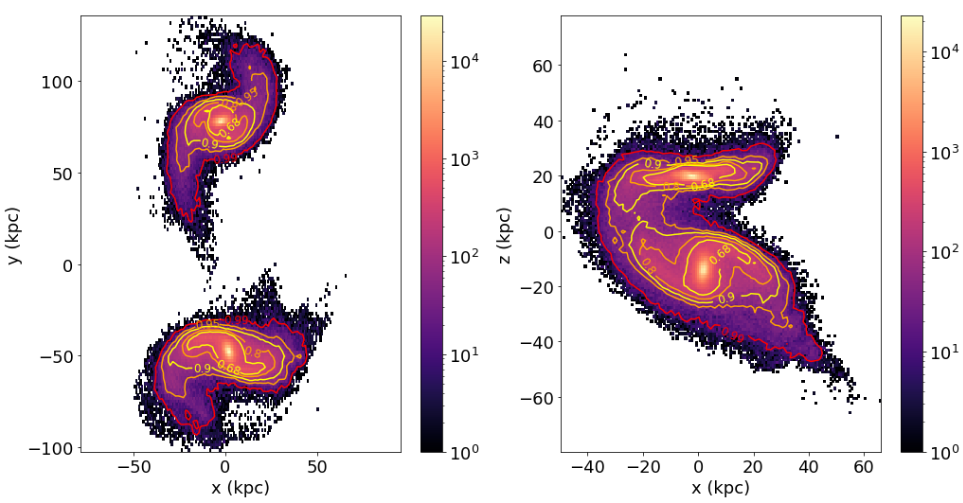
\includegraphics[scale=0.5]{mpl contours, 400b code} \par}

\subsection{Matplotlib plus mpl\_scatter\_density}

This isn't a new problem, so someone wrote an extension to matplotlib to make density plots easier.

Website: \url{https://github.com/astrofrog/mpl-scatter-density}

Borrowing heavily from their examples, this is a first attempt:

\lstdefinestyle{py}{
	belowcaptionskip=1\baselineskip,
	breaklines=true,
	frame=L,
	xleftmargin=\parindent,
	language=Python,
	showstringspaces=false,
	basicstyle=\footnotesize\ttfamily,
	keywordstyle=\bfseries\color{green!40!black},
	commentstyle=\itshape\color{purple!40!black},
	identifierstyle=\color{blue},
	stringstyle=\color{orange},
}

\lstset{style=py} 
\begin{lstlisting}
# install with `conda install mpl-scatter-density`
import mpl_scatter_density

# Make the norm object to define the image stretch
from astropy.visualization import LogStretch
from astropy.visualization.mpl_normalize import ImageNormalize
norm = ImageNormalize(vmin=0., vmax=1000, stretch=LogStretch())

# Make the plot in the (almost) usual pyplot way
# Note the projection to invoke mpl_scatter_density
#  and the norm to use LogStretch

fig = plt.figure(figsize=(12,10))
ax = fig.add_subplot(1, 1, 1, projection='scatter_density')
density = ax.scatter_density(disks[0], disks[1], norm=norm)
plt.xlim(-120, 120)
plt.ylim(-120, 120)

# Add axis labels (standard pyplot)
fontsize = 18
plt.xlabel('x (kpc)', fontsize=fontsize)
plt.ylabel('y (kpc)', fontsize=fontsize)
fig.colorbar(density, label='Number of stars per pixel')
\end{lstlisting}

{\centering 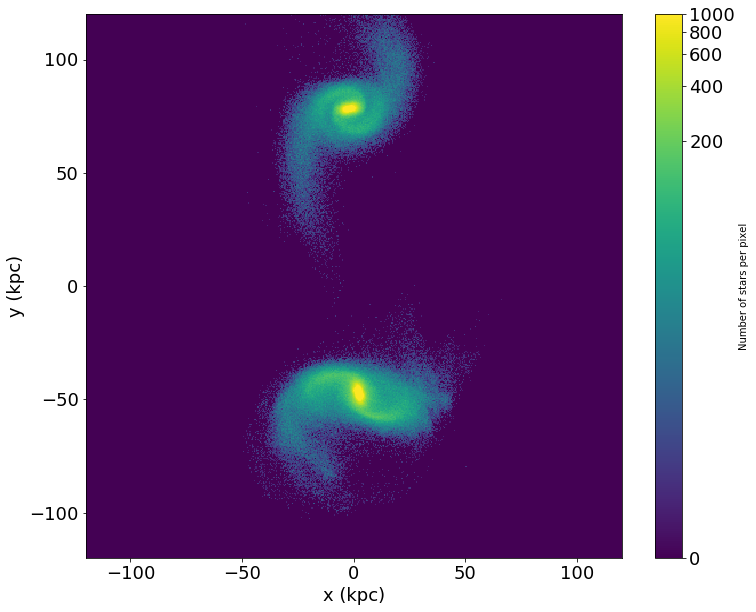
\includegraphics[scale=0.55]{msg} \par}

The colorbar needs some work, but we now get pixel-level resolution. It's a bit easier to see the tidal tails, at least on screen (printouts can be disappointing).

\section{Interactive plots}

Getting away from matplotlib, there are some newer\footnote{In other words, typically less finished and poorly documented} options which use the power of modern graphics cards to handle large numbers of points. More powerful, steeper learning curve.

\subsection{datashader}

Websites: \url{https://github.com/holoviz/datashader} and \url{https://datashader.org}

This needs the data to be arrange columnwise in a (single) pandas dataframe; fairly typical for modern plotting packages. Used in isolation, datashader will make a 2D image. To add axes, labels, etc, it needs to be hooked into a suitable browser-based package such as Bokeh (usually) or Plotly (under development). This can mean a LOT of extra packages to install from conda or pip and lots of potential conflicts\footnote{The release of Bokeh 2.0 broke datashader 0.10.0. For now, use Bokeh 1.4.0 and hope datashader 0.13 is released soon. The developer says he's working on it while in self-isolation after flying home from Covid-hit Spain.}


\subsection{ipyvolume}

Works natively with 3D data. Only in the browser as it relies on WebGL rendering.

Websites: \url{https://github.com/maartenbreddels/ipyvolume} and  \url{https://ipyvolume.readthedocs.io/en/latest/}

Spectacular when the developer (Maarten Breddels, a Dutch astronomer) demonstrates it at conferences, not so easy for the rest of us.

\subsection{All things OpenGL}

Now we're at the heavy end of the options. With pyqt5 + (pyopengl or vispy), an experienced graphics programmer with unlimited time can do virtually anything.

I played with this a bit over spring break. At the current rate of progress, I may have a crude prototype working by the end of the Spring 2021 semester (but no promises).

\end{document}
